\section{Introduction}
The goal of our project was to make the \emph{Beer Framework} more secure.
In order to do that we integrate it with the \emph{SKNX} with \emph{Multiparty Key Agreement Scheme} and \emph{\color{red} Algorithm} encryption algorithm.

\subsection{Beer Framework}
\emph{" The purpose of BeeR is to extend the capabilities of the MANGO framework
	to allow distributed embedded devices, connected together through the network,
	to participate in the execution of an application. With this approach, an application
	can choose to execute its tasks leveraging CPU-based general purpose
	nodes scattered across the network, or reserve only a subset of the tasks for remote
	computation and launching the remaining ones on heterogeneous nodes
	connected through the PCI express link. This means that client applications are
	able to communicate with remote entities, where an instance of the BeeR daemon
	is in execution. This has to be done transparently by the MANGO library,
	without modifying its existing interface.
	It is clear that in order to achieve this goal, a client-server architecture should
	be adopted. Client needs a way to discern if any of the tasks is running on a
	local node, or is going to be run in a remote one. In this way during the resource
	allocation stage it is possible to differentiate between local and remote resources,
	and act consequently. Furthermore, client should be able to replicate most of the
	data structure on the remote device, by sending and receiving data wrapped into
	messages, which of course require the definition of a protocol. On the other hand,
	server must be able to replicate the work-flow of a typical mango application,
	such as allocate buffers and kernels, execute the kernel, wait for events, read and
	write buffers. Client application should take into account the architecture of the
	server and correctly provide a pre-compiled binary executable. Since we could
	have multiple MANGO application running at the same time on different hosts,
	and different devices, BeeR follows a Many-To-Many structure, meaning that
	each instance of the server could receive tasks from multiple client applications. "}\\

\begin{figure}[h]
	\centering
	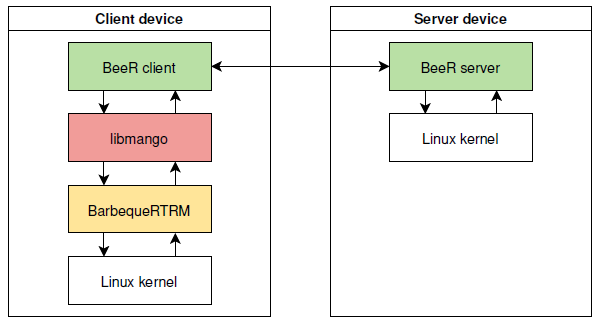
\includegraphics[scale=0.8]{Images/Diagrams/Beer_Devices}
	\caption{Beer Devices Types}
\end{figure}

\subsubsection{Beer Client}
\emph{" The BeeR client is a typical MANGO application, leveraging the set of libraries
	provided by the framework, as shown in Figure 1. To provide the capability
	of offloading tasks and buffers to a remote BeeR server instance, the underlying
	libmango was extended. "}

\subsubsection{Beer Server}
\emph{" The BeeR server is the component of the framework in charge of managing
	the execution of a kernel on a device, as remotely required from a "host"
	machine. The server is executed as a daemon and it does not need to link the
	MANGO library. "}

\subsection{SKNX - Securing Konnex protocol}
\emph{" The Core is a non-blocking DFSA, shown in Figure 1, it starts from the OF-
	FLINE status and for each update(); call, it does some work and updates its
	status. There are 5 states: OFFLINE, COUNTING, HANDSHAKING, FINALIZING,
	ONLINE. If the automata is in ONLINE status, we have completed the key
	handshake.
	At rst, the FSA is in the OFFLINE status. The init() call will change
	the status to COUNTING and start the node counter. When the node counter
	completes its work, the FSA changes its status to HANDSHAKING, it initializes
	the handshake class and and waits for completion. When it is completed,
	there are usually some packets in the output queue that should be sent. This
	is FINALIZING status for. When the output queue is empty, the status is
	changed to ONLINE. If in the whole process there is an error, the FSA jumps
	to OFFLINE. "}
\begin{figure}[h]
	\vspace{1cm}
	\centering
	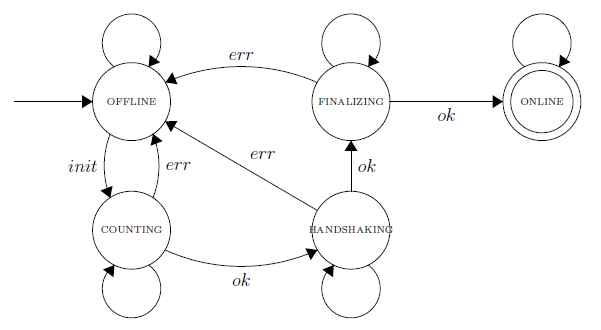
\includegraphics[scale=0.8]{Images/Diagrams/SKNX_states}
	\caption{SKNX Finite State Automata}
\end{figure}